%=======================02-713 LaTeX template, following the 15-210 template==================
%
% You don't need to use LaTeX or this template, but you must turn your homework in as
% a typeset PDF somehow.
%
% How to use:
%    1. Update your information in section "A" below
%    2. Write your answers in section "B" below. Precede answers for all 
%       parts of a question with the command "\question{n}{desc}" where n is
%       the question number and "desc" is a short, one-line description of 
%       the problem. There is no need to restate the problem.
%    3. If a question has multiple parts, precede the answer to part x with the
%       command "\part{x}".
%    4. If a problem asks you to design an algorithm, use the commands
%       \algorithm, \correctness, \runtime to precede your discussion of the 
%       description of the algorithm, its correctness, and its running time, respectively.
%    5. You can include graphics by using the command \includegraphics{FILENAME}
%
\documentclass[11pt]{article}
\usepackage{amsmath,amssymb,amsthm}
\usepackage{graphicx}
\usepackage[margin=1in]{geometry}
\usepackage{fancyhdr}
\usepackage{listings}
\setlength{\parindent}{0pt}
\setlength{\parskip}{5pt plus 1pt}
\setlength{\headheight}{13.6pt}
\newcommand\question[2]{\vspace{.25in}\hrule\textbf{#1: #2}\vspace{.5em}\hrule\vspace{.10in}}
\renewcommand\part[1]{\vspace{.10in}\textbf{(#1)}}
\newcommand\one{\vspace{.10in}\textbf{One-time password SecureID system: }}
\newcommand\two{\vspace{.10in}\textbf{S/Key system: }}
\newcommand\three{\vspace{.10in}\textbf{Challenge response protocol: }}
\newcommand\al{\vspace{.10in}\textbf{Algorithm: }}
\newcommand\ot{\vspace{.10in}\textbf{Output: }}






\pagestyle{fancyplain}
\lhead{\textbf{\NAME\ (\ANDREWID)}}
\chead{\textbf{ASS\HWNUM}}
\rhead{\today}
\begin{document}\raggedright
%Section A==============Change the values below to match your information==================
\newcommand\NAME{Yao Xiao}  % your name
\newcommand\ANDREWID{2019180015}     % your andrew id
\newcommand\HWNUM{1}              % the homework number
%Section B==============Put your answers to the questions below here=======================

% no need to restate the problem --- the graders know which problem is which,
% but replacing "The First Problem" with a short phrase will help you remember
% which problem this is when you read over your homeworks to study.

\question{1}{The First Problem} 

\part{a} \one\\
SMS is an ideal way to reach the recipient. This ensures confirmation of identity via registered mobile number. The banking industry is a perfect application of OTP SMS provider. All the transactions are money related. Such operations must process using verified details.
The generation of OTP is done through using the gateway using the SMS after they are generated at the server side. The security of OTP is reinforced because both the user platform and mobile number are not vulnerable to attacks at the same time.

\part{b} \two\\
Based on the S/Key system authentication method, the user submits registration data including the user name, password, iteration value, and biometric value to the authentication server through the client when the user first registers. The first one-time password for the password sequence. In the user identity authentication process, two-way authentication is performed between the client and the server, and it is a two-way authentication combining the one-time password and biometric value of the registered user.

\part{b} \three\\
Mysql handshake process, after the client actively initiates the link successfully, the server actively sends a challenge protocol, which contains the seed and the attributes supported by the server.
Then the client sends the response protocol to the server for verification through the seed summary password.

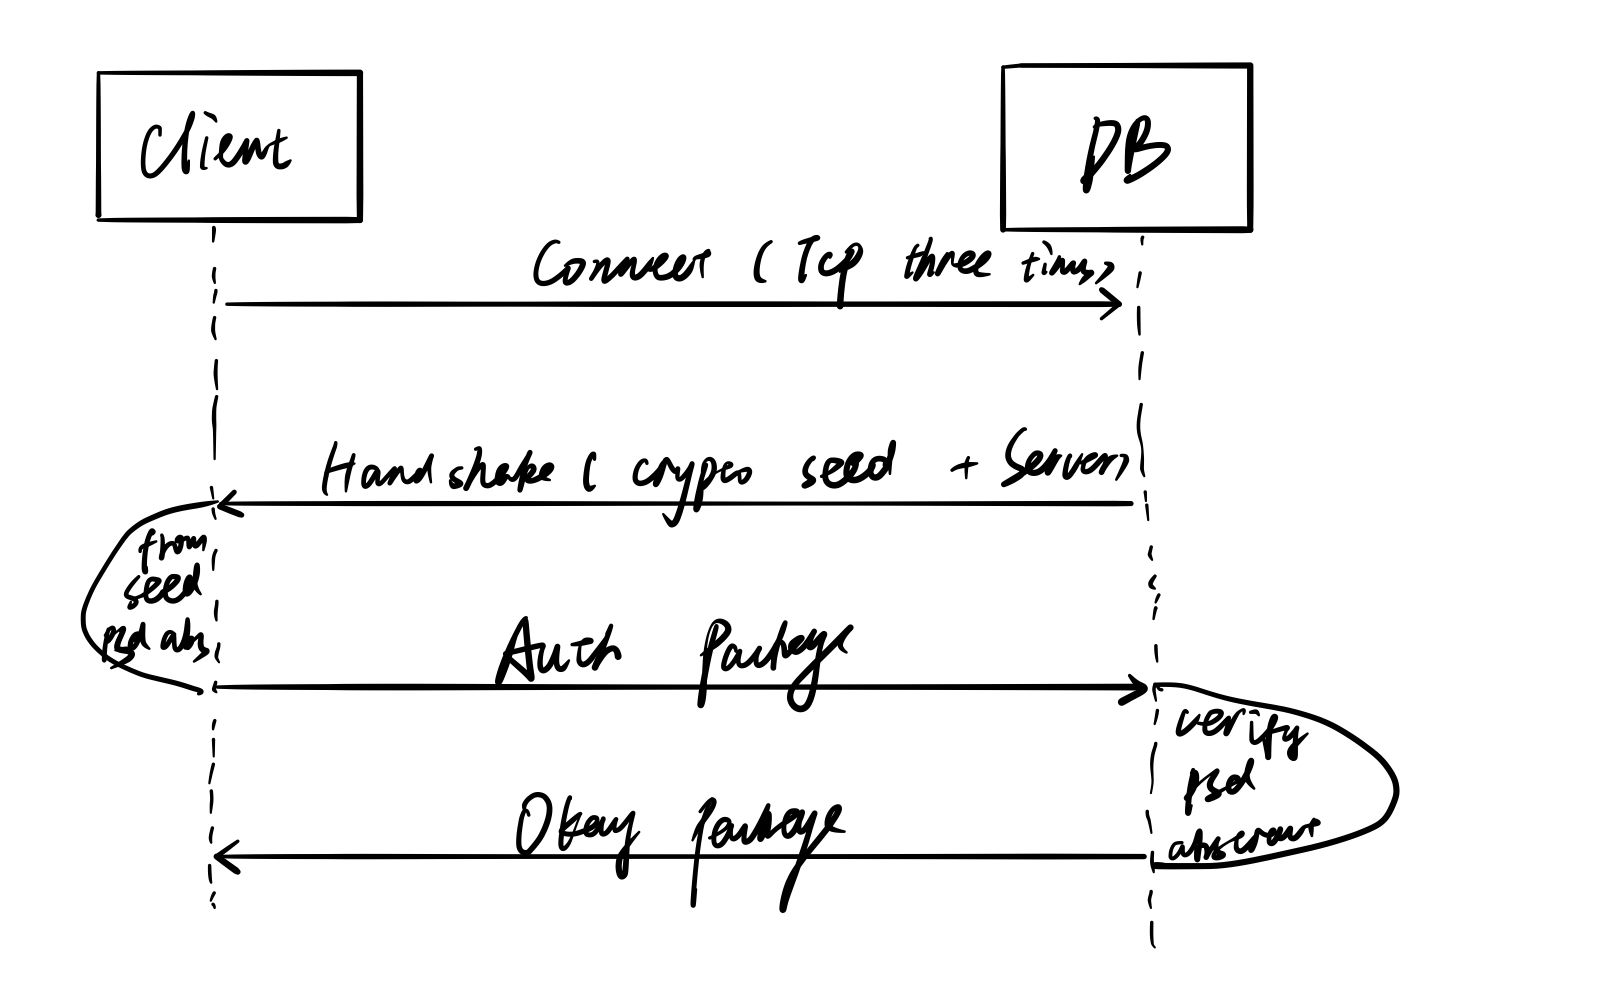
\includegraphics[scale=0.3]{f1.jpeg}


\question{2}{The Second Problem}

\part{a} \al Origin \\ 
\begin{lstlisting}
import time
from fastecdsa import keys
from fastecdsa import curve
from Crypto.Hash import SHA256
cur = curve.P256

def key_gen():
    sk = keys.gen_private_key(cur)
    pk = keys.get_public_key(sk, cur)
    g = cur.G
    return sk, pk, g

def sig(m, sk):
    tmp_k = sk
    k1 = keys.gen_private_key(cur)
    k2 = keys.get_public_key(k1, cur)
    h = SHA256.new()
    x = '{:0{}x}'.format(k2.x, 64)
    y = '{:0{}x}'.format(k2.y, 64)
    h.update(m + bytes(x+y, "ascii"))
    ct = h.hexdigest()
    ot = k1 + tmp_k * int(ct, 16)
    return {'k2':k2, 'ot':ot}

def verify(sign, m, g, pk):
    k2 = sign['k2']
    ot = sign['ot']
    h = SHA256.new()
    x = '{:0{}x}'.format(k2.x, 64)
    y = '{:0{}x}'.format(k2.y, 64)
    h.update(m + bytes(x + y, "ascii"))
    ct = h.hexdigest()
    r1 = g * ot
    r2 = k2 + pk * int(ct, 16)
    if r1 == r2:
        print('verify success!')

begin = time.time()
sk,pk,g = key_gen()
m = b"CSCI468/968 Advanced Network Security, Spring 2020"
sign = {}
sign = sig(m, sk)
verify(sign, m, g, pk)
end = time.time()
print("original time: %f" % (end - begin))
\end{lstlisting}

\ot\\
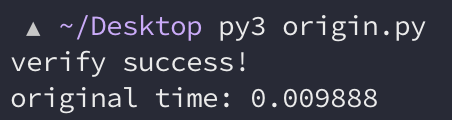
\includegraphics{ot1.png}


\part{b}  \al Optimize\\
\begin{lstlisting}
import time
from fastecdsa import keys
from fastecdsa import curve
from Crypto.Hash import SHA256
cur = curve.P256

def key_gen():
    sk = keys.gen_private_key(cur)
    pk = keys.get_public_key(sk, cur)
    g = cur.G
    return sk, pk, g

def sig(m, sk):
    tmp_k = sk
    k1 = keys.gen_private_key(cur)
    k2 = keys.get_public_key(k1, cur)
    h = SHA256.new()
    x = '{:0{}x}'.format(k2.x, 64)
    y = '{:0{}x}'.format(k2.y, 64)
    h.update(m + bytes(x+y, "ascii"))
    ct = h.hexdigest()
    ot = k1 + tmp_k * int(ct, 16)
    return {'ct':ct, 'ot':ot}

def verify(sign, m, g, pk):
    ct = sign['ct']
    ot = sign['ot']
    h = SHA256.new()
    k2 = g * ot - pk * int(ct, 16)
    x = '{:0{}x}'.format(k2.x, 64)
    y = '{:0{}x}'.format(k2.y, 64) 
    h.update(m + bytes(x + y, "ascii"))
    ct2 = h.hexdigest()
    if ct == ct2:
        print('verify success!')
    else:
        print('verify fail!')

begin = time.time()
sk,pk,g = key_gen()
m = b"CSCI468/968 Advanced Network Security, Spring 2020"
sign = {}
sign = sig(m, sk)
verify(sign, m, g, pk)
end = time.time()
print("optimize time: %f" % (end - begin))
\end{lstlisting}

\ot\\
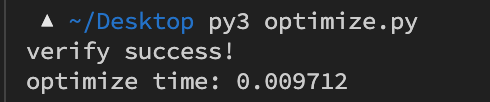
\includegraphics{ot2.png}

\question{3}{The Third Problem}
The derivation process:
\begin{gather}
    a_{z0} = a_{t0} + sk \cdot C_0\\
    a_{z1} = a \cdot a_{t0} + b + sk\\
    c_0 = H(m_0,v_{t0})\\
    v_{t0} = g^{a_{t0}}\\
    c_1 = H(m_1, V_{t1})\\
    v_{t1} = g^{a \cdot a_{t0} + b}\\
    a \cdot a_{z0} + b = a \cdot a_{t0} + b\\
    a_{z1} = a \cdot a_{t0} + b + sk \cdot c_1\\
    sk = \frac{a \cdot a_{z0} + b - a_{z1}}{a \cdot c_0 - c_1}
\end{gather}

\question{4}{The Fourth Problem}
The derivation process:

\begin{align}
    \overline{a} &= \sum_{i=1}^{n}a_{zi}\\
    \overline{c} &= \sum_{i=1}^{n}c_i\\
    &\Rightarrow \frac{\overline{a^1}}{c^1}\\
    \overline{a} &= a_{t0} + sk \cdot \overline{c}\\
    \overline{a^1} &= a_{t0} + sk \cdot \overline{c^1}\\
    &\Rightarrow sk = \frac{\overline{a}-\overline{a^1}}{\overline{c}-\overline{c^1}}
\end{align}


\end{document}
